\section{Campo elettrico}
\subsection{Campo elettrico}

\begin{figure}[h!]
    \centering
    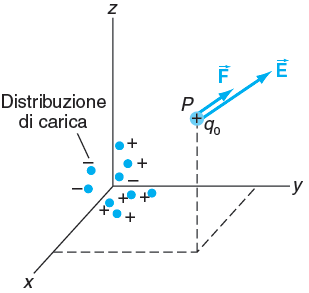
\includegraphics[width=0.3\linewidth]{imgs/1 - campo.png}
    \label{fig:campo}
    \caption{Campo elettrico}
\end{figure}

Il campo elettrico $\vec{E}$ in un punto $P$ dovuto ad un gruppo di particelle è:
\begin{equation}
    \vec{E} = \frac{\vec{F}}{q_0} [\frac{N}{C}]
\end{equation}
Dove $q_0$ è la carica di prova e la si prende piccolissima per non alterare il campo.


A volte si usa una formula più veloce avendo a che fare con tante forze singole.
Si parte dalla formula della forza:
\begin{equation}
    \vec{E} = \frac{1}{4\pi \epsilon_0}\sum{\frac{q_i}{r_i^2}\hat{r_i}}   
\end{equation}

\subsection{Distribuzione continua di cariche}
In base alla distribuzione di carica si hanno tre casi:

\subsubsection{Distribuzione di carica di volume}
$dq = \rho dv$ dove $\rho$ è la densità di carica di volume $[\frac{C}{m^3}]$.

\begin{equation}
    \vec{E} = \frac{1}{4\pi \epsilon_0}\iiint{\frac{\rho}{r^2}\hat{r}dv}
\end{equation}
\subsubsection{Distribuzione di carica di superficie}
$dq = \sigma da$ dove $\sigma$ è la densità di carica di superficie $[\frac{C}{m^2}]$.
\begin{equation}
    \vec{E} = \frac{1}{4\pi \epsilon_0}\iint{\frac{\sigma}{r^2}\hat{r}da}
\end{equation}

\subsubsection{Distribuzione di carica di linea}
$dq = \lambda dl$ dove $\lambda$ è la densità di carica di linea $[\frac{C}{m}]$.

\begin{equation}
    \vec{E} = \frac{1}{4\pi \epsilon_0}\int{\frac{\lambda}{r^2}\hat{r}dl}
\end{equation}

\subsection{Particelle cariche in campo uniforme}
La forza elettrica $\vec{F}=q\vec{E}$, è la froza risultante.
Per la \textbf{seconda legge di Newton}, si ha che $q\vec{E} = m\vec{a}$.
Quindi si ricava che:
\begin{equation}
    \vec{a} = \frac{q\vec{E}}{m}
\end{equation}

\subsubsection{Caso particolare 1}
Particella carica inizialmente in quiete in un campo elettrico uniforme.
Si muove con accelerazione costante lungo una retta parallela a $\vec{E}$.

\begin{center}
    \begin{tabular}{|c|c|c|}
        \hline 
        $a_x=\frac{qE}{m}$ & $V_x = \frac{qE}{m}t$ & $x = \frac{1}{2}\frac{qE}{m}t^2$ \\ [0.5ex]
        \hline
    \end{tabular}
\end{center}
Due casi derivati sono:
\begin{itemize}
    \item $V_x^2 = \frac{2qE}{m}x$
    \item $V_x^2 = (\frac{qE}{m})^2t^2$
\end{itemize}

\subsubsection{Caso particolare 2}
Particella carica che entra con velocità $\vec{v_0}$ in una regione sede di campo uniforme $\vec{E}$ con $\vec{v_0}$ perpendicolare a $\vec{E}$.


\begin{center}
    \begin{tabular}{|c|c|c|}
        \hline 
        $a_y=\frac{qE}{m}$ & $a_x = 0$ & $a_z = 0$ \\ [0.5ex]
        \hline
        $v_y=\frac{qE}{m}t$ & $v_x = v_0$ & $v_z = 0$ \\ [0.5ex]
        \hline
        $y=\frac{1}{2}\frac{qE}{m}t^2$ & $x = v_0 t$ & $z = 0$ \\ [0.5ex]
        \hline
    \end{tabular}
\end{center}

\begin{figure}[H]
    \centering
    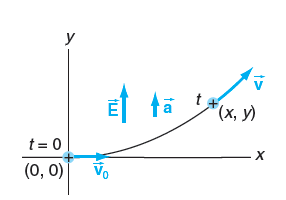
\includegraphics[width=0.3\linewidth]{imgs/2 - moto di proiettile.png}
    \label{fig:moto_parabolico}
    \caption{Moto con traiettoria parabolica}
\end{figure}
Formula del moto parabolico:
\begin{equation}
    y = \frac{1}{2}\frac{qE}{mv_0^2}x^2
\end{equation}

